\section{Method 2: GANs \& FOMM}

% --- Slide 1: Standard GAN ---
\begin{frame}{Standard GAN Architecture}
    \begin{columns}[c]
        \begin{column}{0.48\textwidth}
            \textbf{How GANs Work (Goodfellow et al., 2014)}
            \begin{itemize}
                \item Two neural networks competing against each other in an adversarial setup:
                \item \textbf{Generator ($G$):} Takes a random noise vector $\mathbf{z}$ and learns to synthesize realistic facial images.
                \item \textbf{Discriminator ($D$):} Evaluates images and classifies them as real (from dataset) or fake (from $G$).
                \item \textbf{Adversarial training:} Through gradient feedback, $G$ progressively captures fine details and photorealistic textures.
            \end{itemize}
        \end{column}

        \begin{column}{0.50\textwidth}
            \centering
            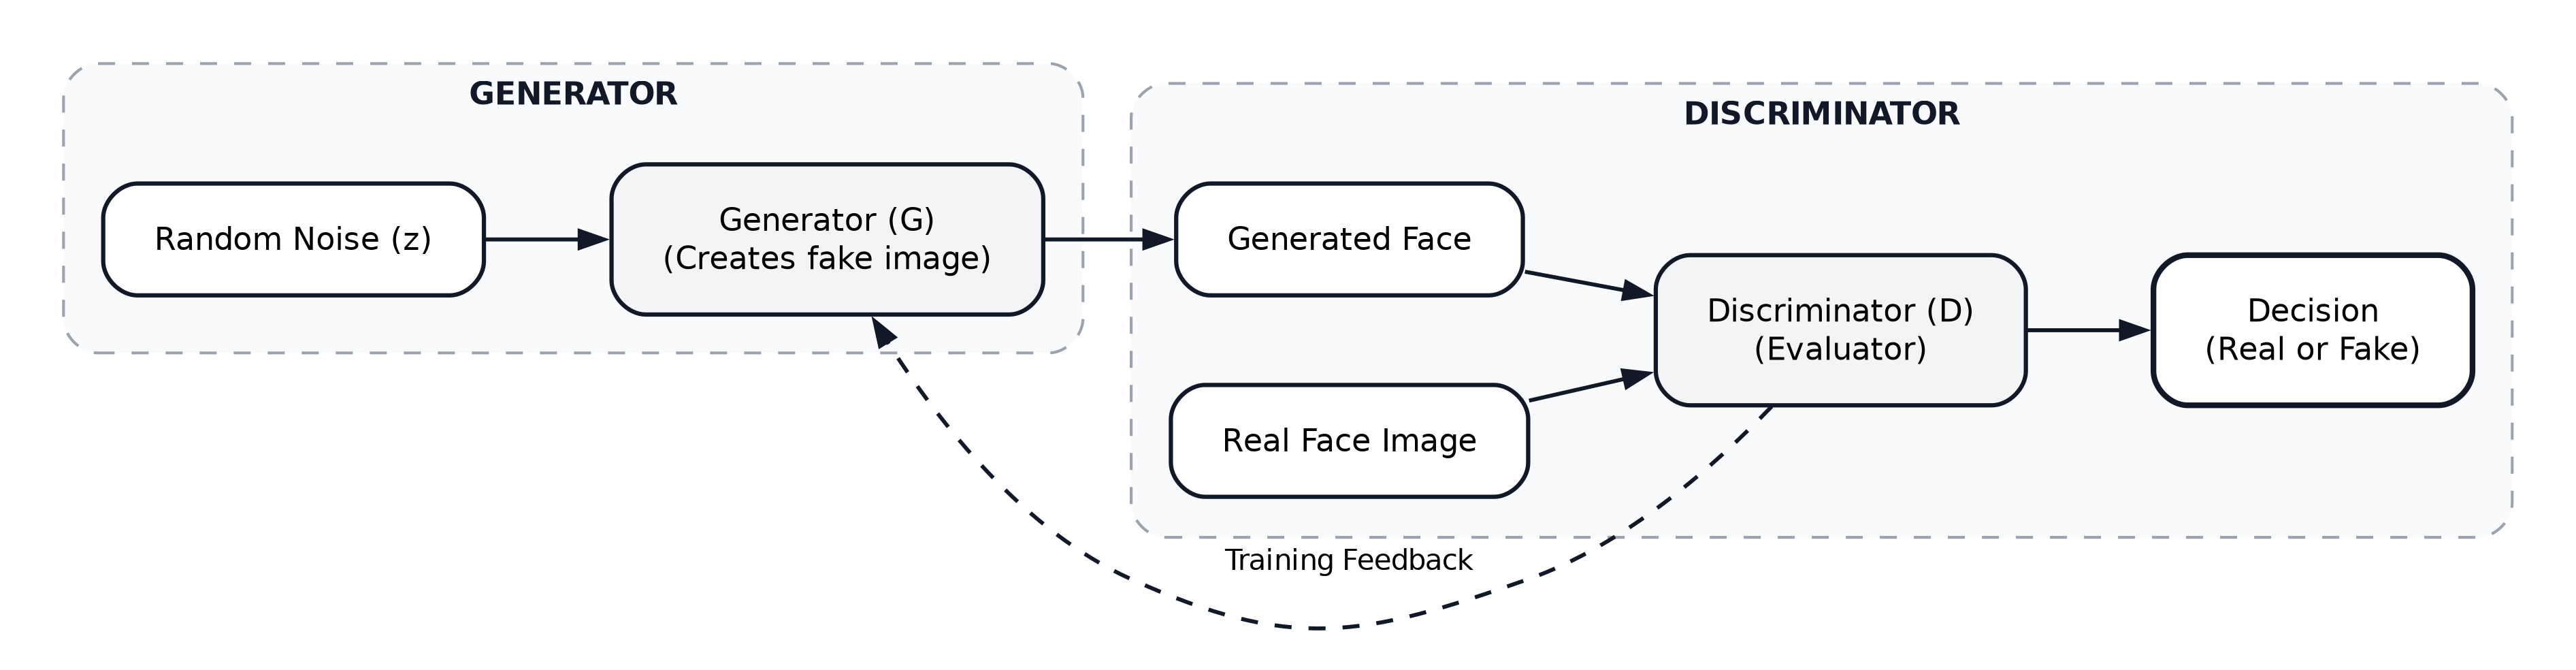
\includegraphics[width=\linewidth, height=4.2cm, keepaspectratio]{diagram_standard_gan.png}
        \end{column}
    \end{columns}
\end{frame}

% --- Slide 2: Why Standard GANs Fail ---
\begin{frame}{The Controllability Issue in Vanilla GANs}
    \begin{columns}[c]
        \begin{column}{0.50\textwidth}
            \begin{block}{Why Unconditional GANs Fall Short}
                \small
                \begin{itemize}
                    \item Generates arbitrary faces from random noise $\mathbf{z}$.
                    \item Identity, pose, and emotion are entangled in latent space.
                    \item Cannot say: \textit{"keep Person A, copy Person B's expression"}.
                \end{itemize}
            \end{block}
            
            \begin{block}{What Face Reenactment Requires}
                \small
                \begin{itemize}
                    \item \textbf{Identity conditioning:} Appearance anchored strictly to source portrait $S$.
                    \item \textbf{Motion conditioning:} Facial dynamics driven frame-by-frame by driving video $D$.
                \end{itemize}
            \end{block}
        \end{column}

        \begin{column}{0.48\textwidth}
            \centering
            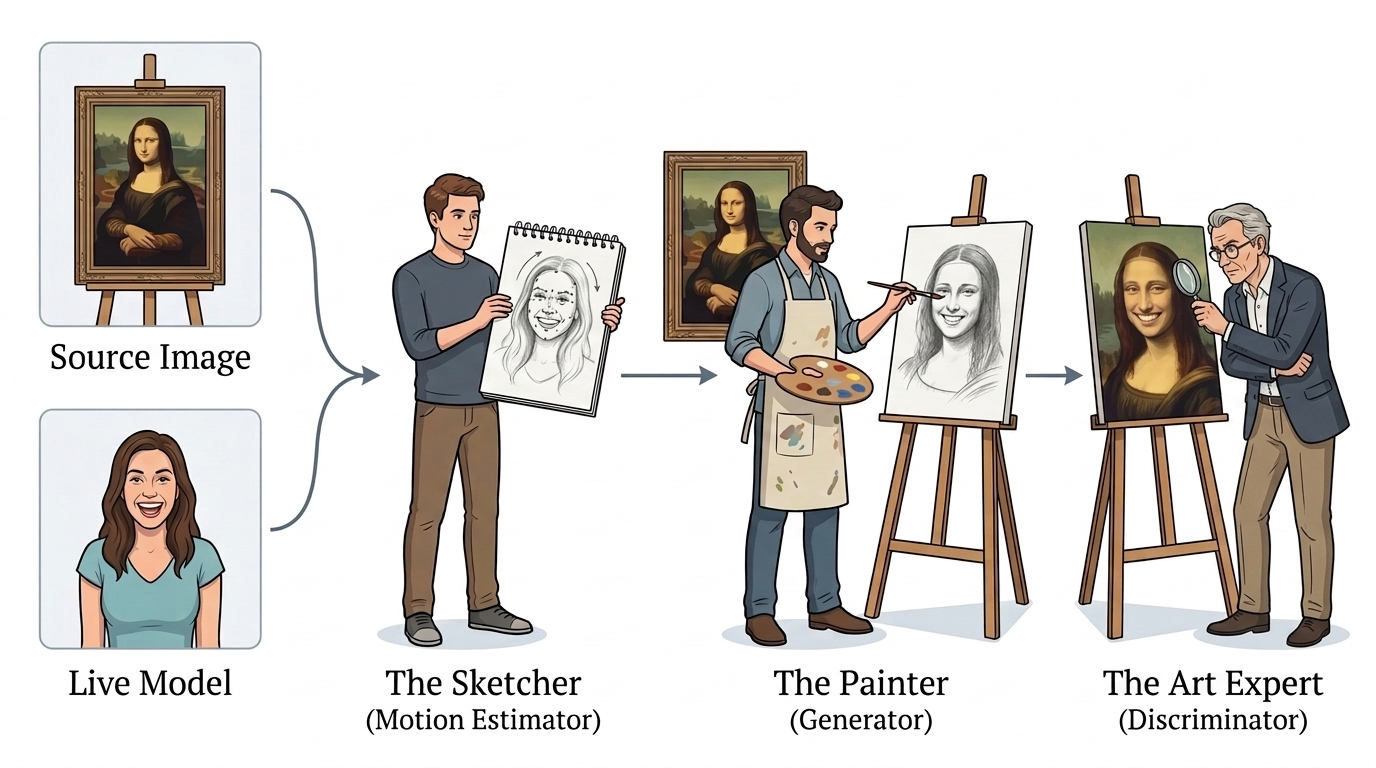
\includegraphics[width=\linewidth, keepaspectratio]{ressam_dedektif_analoji.png}
        \end{column}
    \end{columns}
\end{frame}
